\section{Aplicación Web para la Visualización y Prueba del Modelo}
\label{ap:AplicacionWeb}
Como culminación del presente Trabajo de Fin de Máster, se ha desarrollado y desplegado una aplicación web interactiva que ejecuta el sistema multimodal completo (\textit{Ensemble} mediante \textit{Late Fusion}). Esta herramienta permite clasificar nuevas instancias de vídeo en tiempo real. 

Para superar las limitaciones de memoria VRAM (15 GB) de los entornos gratuitos y evitar el colapso del sistema, se ha diseñado una arquitectura inteligente de carga secuencial y liberación dinámica de memoria. Esto permite ejecutar iterativamente modelos masivos que, en un despliegue estático tradicional, requerirían infraestructura de alto coste.  

\section*{Arquitectura y Tecnologías Utilizadas}
Para hacer viable el despliegue del sistema \textit{Ensemble} completo (combinando \textit{Mistral}, \textit{ConvNeXt} y \textit{TimeSFormer}), la aplicación utiliza una arquitectura puente que separa el \textit{backend} de cómputo del \textit{frontend} de visualización:
\begin{itemize}
    \item \textbf{Backend y Cómputo (\textit{Google Colab})}: El núcleo de procesamiento se ejecuta en un entorno de \textit{Google Colab} equipado con una \textit{GPU NVIDIA T4}, montando \textit{Google Drive} para la carga local de los pesos de los modelos. Aquí se ejecuta la lógica pesada y la cuantización de \textit{Mistral-7B} en 4-bits mediante \textit{QLoRA}.
    \item \textbf{Túnel de Conexión (\textit{Gradio})}: Mediante la librería \textit{Gradio}, el entorno de Colab genera un túnel inverso temporal (URL pública \texttt{.gradio.live}) que expone la interfaz interactiva hacia el exterior.
    \item \textbf{Frontend Estático (\textit{Hugging Face Spaces})}: Para dotar al proyecto de una URL institucional y permanente, se ha habilitado un \textit{Space} en \textit{Hugging Face}. Dicho espacio funciona como un contenedor estático (mediante un archivo \texttt{index.html}) que embebe la interfaz generada por Colab. Por tanto, el cómputo masivo no recae sobre los limitados servidores de Hugging Face, sino sobre la GPU de Google.
\end{itemize}

Esta arquitectura implica que la disponibilidad de la aplicación está sujeta a que el cuaderno de ejecución en \textit{Google Colab} se encuentre activo.

\section*{Acceso a la Aplicación y Código Fuente}
La herramienta se encuentra vinculada para su visualización desde cualquier navegador web estándar en la siguiente URL:

\begin{center}
\textbf{\url{https://huggingface.co/spaces/visumania2/DeepSexist-App}}
\end{center}

Asimismo, con el fin de garantizar la transparencia y reproducibilidad de esta investigación, el código fuente completo del proyecto está alojado en un repositorio público. Este repositorio contiene los cuadernos de entrenamiento originales (incluyendo el historial de versiones), los \textit{scripts} de gestión del \textit{dataset} y los cuadernos de despliegue de esta misma aplicación (omitiendo los datos audiovisuales restringidos por la competición):
\begin{center}
\textbf{\url{https://github.com/visumania/DeepSexist}}
\end{center}

\section*{Manual de Usuario}
El uso de la aplicación consta del siguiente flujo simplificado:

\begin{enumerate}
    \item Acceder a la URL habilitada.
    \item Cargar un archivo de vídeo (\texttt{.mp4}, \texttt{.avi}) en el componente principal de la pantalla. 
    \item Pulsar el botón ``Ejecutar Pipeline Multimodal''.
    \item El sistema procesará de forma automatizada las vías requeridas: transcripción de audio a texto, \textit{mean-pooling} de 4 fotogramas visuales y análisis de la matriz del movimiento. 
    \item Tras el procesado, se visualizarán las probabilidades de sexismo independientes de cada modelo y el resultado final calculado por la suma ponderada del \textit{Ensemble} (35\% texto, 55\% imagen y 10\% vídeo).
\end{enumerate}

\section*{Ejemplo de Uso}
A continuación, se detalla un caso de uso práctico procesado por el \textit{Ensemble}:
\begin{itemize}
    \item \textbf{Vídeo introducido}: Clip de 15 segundos con un discurso basado en roles tradicionales. 
    \item \textbf{Transcripción automática (\textit{Whisper})}: ``\textit{El lugar de las mujeres está en casa, no en una oficina dirigiendo empresas}''. 
    \item \textbf{Modelo Texto (\textit{Mistral}-35\%)}: Probabilidad de Sexismo: 98.20\%.
    \item \textbf{Modelo Imagen (\textit{ConvNeXt}-55\%)}: Probabilidad de Sexismo: 62.40\%.
    \item \textbf{Modelo Vídeo (\textit{TimeSFormer}-10\%)}: Probabilidad de Sexismo: 71.00\%.
    \item \textbf{Resultado Final (\textit{Ensemble})}: Probabilidad del \textit{Ensemble}:75.79\%. Resultado final: \textbf{SEXISTA}.
\end{itemize}

\section*{Capturas de Pantalla}

A continuación, en la \autoref{fig:CapturaGradio} se muestra el aspecto visual de la aplicación web en funcionamiento:

\begin{figure}[H]
    \centering
    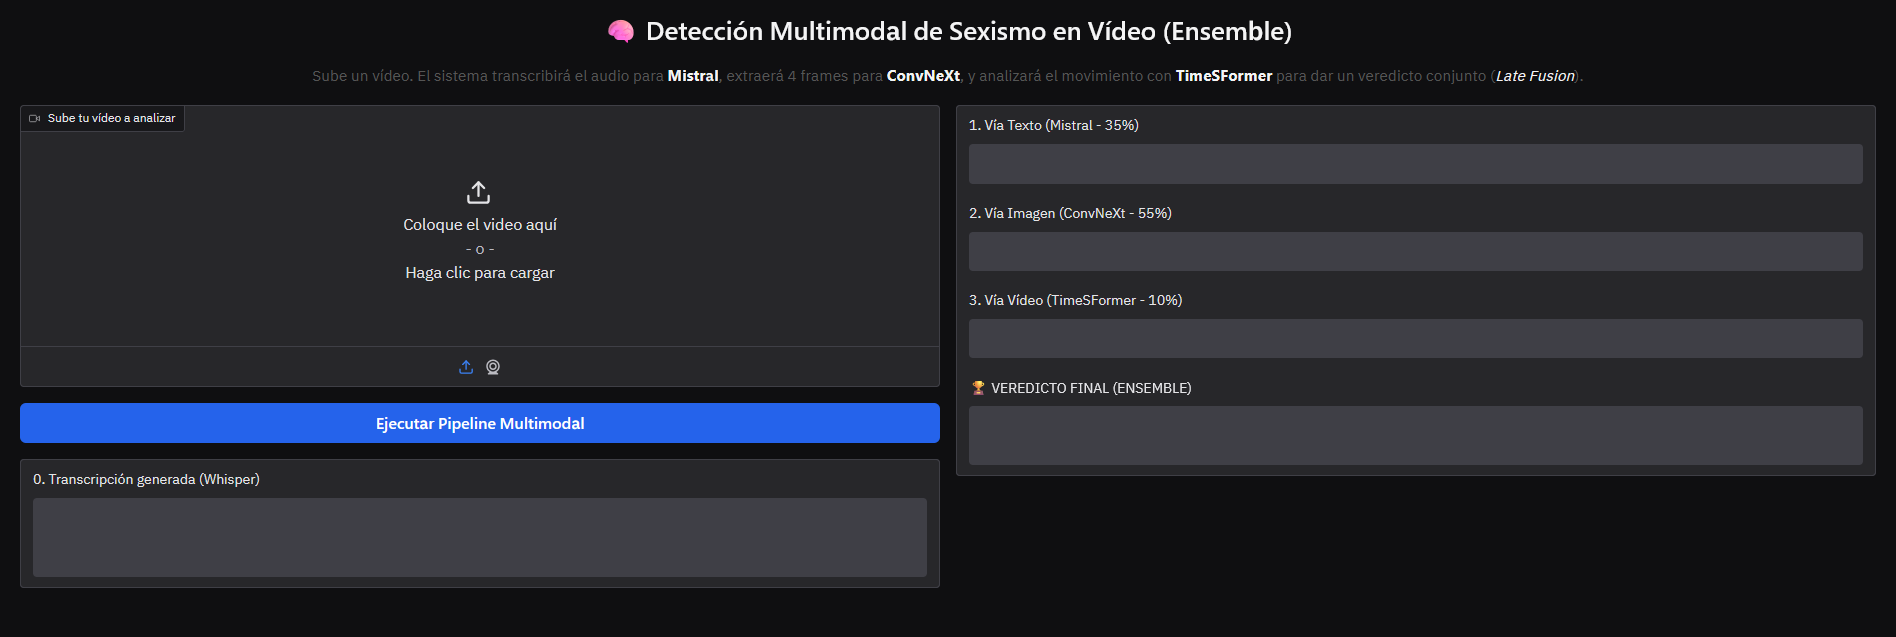
\includegraphics[width=1\textwidth]{Figuras/CapturaGradio.png}
    \caption{Interfaz web desarrollada con Gradio alojada mediante un \textit{iframe} en \textit{Hugging Face Spaces}.}
    \label{fig:CapturaGradio}
\end{figure}